\chapter{Figures for Preparation}

% Structure sets spectrum
\begin{figure}[ht]
    \centering
    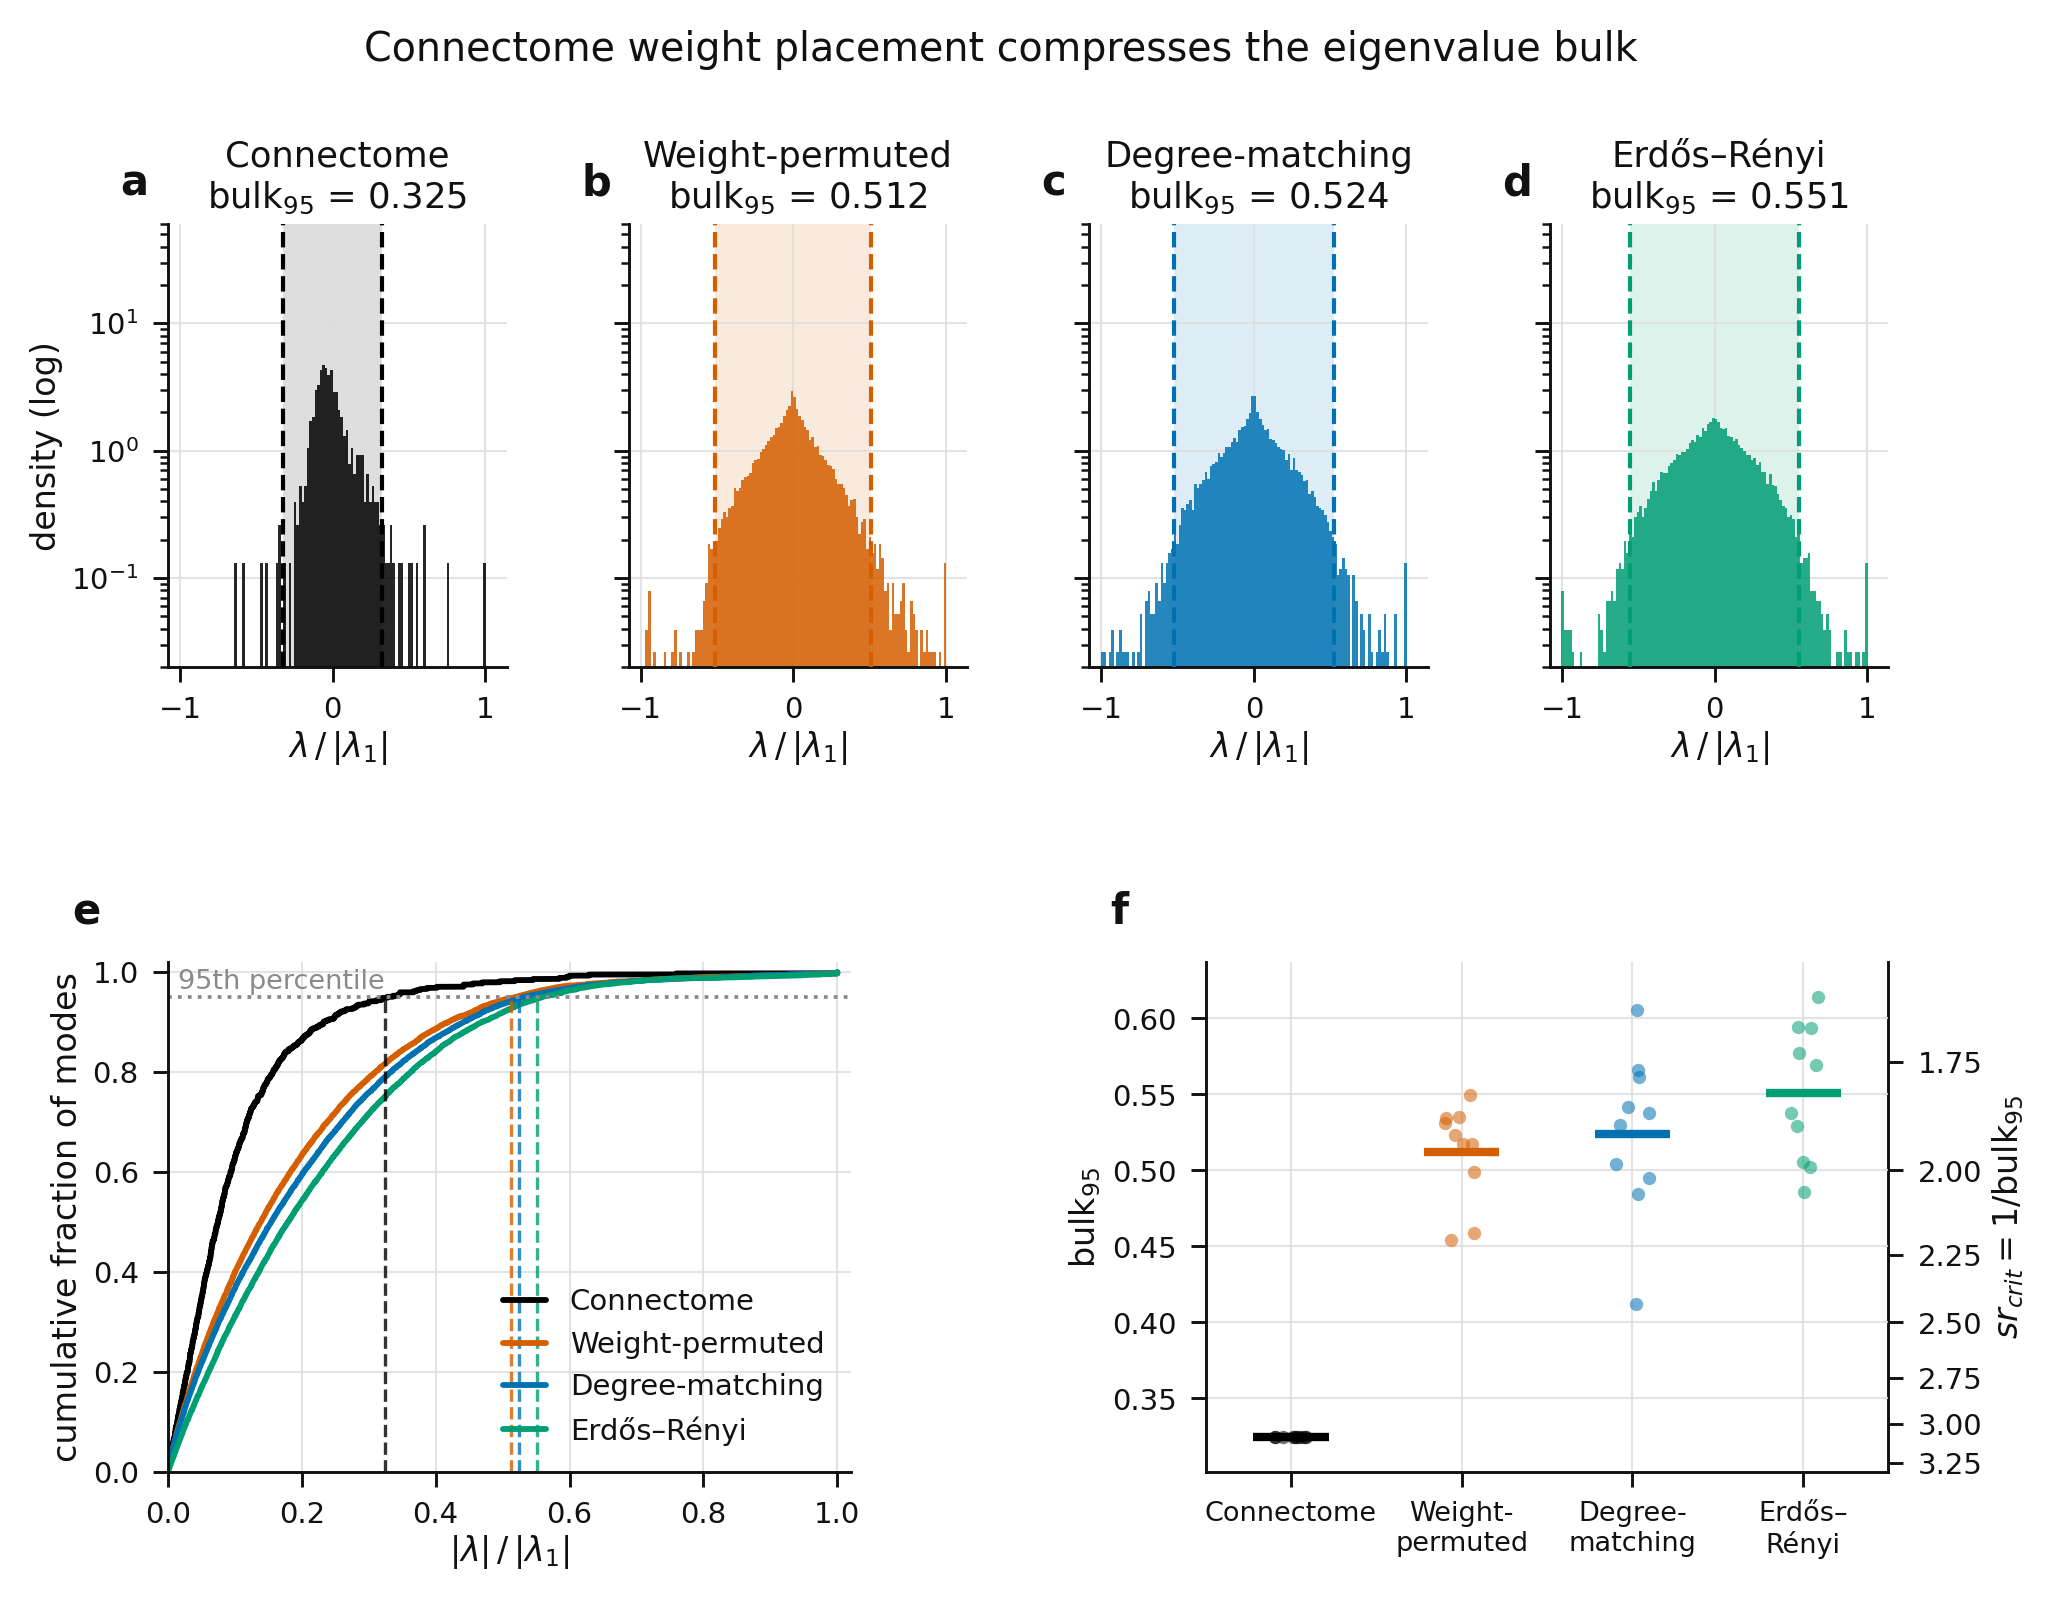
\includegraphics[width=\textwidth]{figures/fig1_structure_sets_spectrum.png}
    \caption[Structure sets spectrum]{\textbf{Connectome weight placement compresses the eigenvalue bulk:} Spectra of the recurrent matrix W for the human structural connectome and three controls, human SC consensus, N = 448, 10 seeds per variant. Every panel is drawn on the normalised matrix, the object the reservoir build actually rescales, so the leading eigenvalue sits at 1 by construction and all quantities are scale-invariant ratios.}
    \label{fig:structure-sets-function}
\end{figure}




\newpage
\section{Problem Statement}
\label{section:problem}
\bigskip

% Emphasize need for a novel intuitive robot control method
% Imagined interaction

Humans instinctively and innately engage with their surroundings through physical interaction, grasping, manipulating, and manoeuvring objects with their hands and bodies. This natural inclination, rooted in our biological makeup, is essential for survival and understanding the world. Brain-computer interfaces (BCIs) leverage this ability for motor imagery, mentally rehearsing physical actions, to bypass traditional motor pathways and offer new avenues for restoring independence and enhancing capabilities for individuals with motor impairments.
However, current motor imagery (MI)-BCI designs for robotic manipulator control lack intuitiveness, relying on single-body part activation unnatural to users, as the imagined movements do not correspond directly with the resulting robotic arm motions. Consequently, extensive training is required, limiting real-world deployment possibilities. This study explores redesigning MI-BCIs based on \say{imagined interaction}, where subjects imagine physically engaging and manipulating the robotic arm in free space, contrasting with the traditional imagining of hand or foot movements.



\section{Research Questions}
\label{section:questions}
\bigskip

% Small intro describing how the problem statement has influenced the research questions...

\begin{enumerate}
    \item To what extent can the direction of imagined manipulation with a robotic arm be predicted from the EEG signals recorded during interaction?
    \item How accurately can the direction of imagined manipulation for other cognitive tasks involved in robotic interaction be predicted and how do their performances compare? The tasks include:
    \begin{itemize}
        \item \textbf{Motor execution}: user physically moves the robot using both arms
        \item \textbf{Visual perception}: user observes the motion of the robot in front of them
        \item \textbf{Motor imagery}: user imagines moving the robot using both arms
        \item \textbf{Motor imagery during visual perception}: user imagines moving the robot while observing its motion at the same time.
    \end{itemize}
    \item Which computational methods designed for EEG classification perform best for decoding signals during robotic arm interaction, and why might certain model architectures or training procedures yield better results?
    \item What neurophysiological features can be learned from analysis of the EEG signals obtained across the various tasks, and how can these inform future research in neuroscience?
\end{enumerate}



\section{Aims and Objectives}
\label{section:Aims}
\bigskip

This study aims to propose a novel BCI paradigm for recording EEG data during intuitive (imagined and executed) interaction with a robotic arm. Furthermore, it aims to evaluate the classification performance of state-of-the-art (SOTA) machine learning (ML) and deep learning (DL) models in decoding manipulation intent. The results of the work hold the potential to improve the quality of human-robot interaction in BCIs and to shed light on the neurophysiological processes during both real and imagined robotic manipulation.
\\\\
Project objectives include:
\begin{enumerate}
    \item Define a novel experimental paradigm for intuitive robotic interaction
    \item Collect EEG recordings from at least 10 subjects engaging in the paradigm
    \item Preprocess the data and remove both environmental and biological artifacts
    \item Perform detailed analysis on signals in the form of frequency bands, event-related spectral pertubations (ERSPs), and motion-onset visual evoked potentials (mVEPs)
    \item Reproduce 4 SOTA EEG classification models and train them on labelled recordings for binary classification of motion direction
    \item Propose 1 novel classification model based on prior neuro-scientific knowledge. Similarly, train on labelled recordings for binary classification of motion direction
    \item Evaluate the models by performing k-fold cross validation (k=10), using test accuracy and F1-score as evaluation metrics
\end{enumerate}



% \section{Anticipated Outputs}
% \label{section:outputs}
% \bigskip


\afterpage{\blankpage}
